%
% $Id: slides.tex 4228 2006-06-21 21:55:12Z jjamor $
%
%
% Compilar a .pdf con LaTeX (pdflatex)
% Es necesario instalar Beamer (paquete latex-beamer en Debian)
%

%
% Gráficos:
% Los gráficos pueden suministrarse en PNG, JPG, TIF, PDF, MPS
% Los EPS deben convertirse a PDF (usar epstopdf)
%

\documentclass{beamer}
\usetheme{Warsaw}
\usebackgroundtemplate{
\includegraphics[width=\paperwidth]{format/libresoft-bg.png}}
\usepackage[spanish]{babel}
\usepackage[utf8]{inputenc}
\usepackage{graphics}
\usepackage{amssymb} % Simbolos matematicos
\usepackage{url}

%\definecolor{libresoftgreen}{RGB}{162,190,43}
%\definecolor{libresoftblue}{RGB}{0,98,143}

%\setbeamercolor{titlelike}{bg=libresoftgreen}

%% Metadatos del PDF.
\hypersetup{
  pdftitle={Introduction to ISO 9126},
  pdfauthor={F. Ortega, D. Izquierdo, P. Coca},
  pdfcreator={GSyC/Libresoft},
  pdfproducer=PDFLaTeX,
  pdfsubject={nn},
}
%%


\AtBeginSection[]
{
  \begin{frame}<presentation>
    \frametitle{Index}
    \tableofcontents[current]
  \end{frame}
}


\begin{document}

\title{Introduction to ISO 9126}
\subtitle{Master on Free Software}
\institute{\\jfelipe@libresoft.es\\
GSyC/Libresoft}
\author{Felipe Ortega, Daniel Izquierdo, Pedro Coca}
\date{\today}

\frame{
\maketitle
\begin{center}

\includegraphics[width=6cm]{format/gsyc-urjc}
\end{center}
}


% Si el titulo o el autor se quieren acortar para los pies de página
% se pueden redefinir aquí:
%\title{Titulo corto}
%\author{Autores abreviado}


%% LICENCIA DE REDISTRIBUCION DE LAS TRANSPAS
\frame{
~
\vspace{4cm}

\begin{flushright}
{\tiny
(cc) 2010 Felipe Ortega, Daniel Izquierdo, Pedro Coca. \\
Some rights reserved. This document is distributed under the Creative \\
            Commons Attribution-ShareAlike 3.0 licence, available in \\
            http://creativecommons.org/licenses/by-sa/3.0/

%  Este documento (o uno muy similar) está disponible en \\
%  \url{http://gsyc.escet.urjc.es/~jjamor/}
}
\end{flushright}
}
%%

%%%%%%
%Transpas separadas por \begin{frame}
%%%%%%%%%%%%%%%%%%%%%%%%\end{frame}

\section{Introduction}

\begin{frame}
\frametitle{What is ISO?}
\begin{itemize}
\item ISO: International Organization for Standardization 
\item One of the largest organizations in charge of developing and publishing standards
\item There are at least 160 different countries
\item \url{http://www.iso.org/iso/home.htm}
\end{itemize}
\end{frame}

%%%%%%%%%%%%%%%%%%%%%%%%%%%%%%%%%%%%%%%%%%%%%%%%%%%%%%%%%%%%%%

\begin{frame}
 \frametitle{ISO 9126}
 \begin{itemize}
 \item Full name: ISO 9126-1 Software engineering -- Product quality -- Part 1: Quality model 
 \item This model is based on six main attributes
 \item and 27 sub-attributes
 \end{itemize}
\end{frame}

%%%%%%%%%%%%%%%%%%%%%%%%%%%%%%%%%%%%%%%%%%%%%%%%%%%%%%%%%%%%%%

\begin{frame}
 \frametitle{Main attributes}
 \begin{itemize}
  \item Functionality
  \item Reliability
  \item Usability
  \item Efficiency
  \item Maintainability
  \item Portability
 \end{itemize}
\end{frame}

%%%%%%%%%%%%%%%%%%%%%%%%%%%%%%%%%%%%%%%%%%%%%%%%%%%%%%%%%%%%%%

\begin{frame}
 \frametitle{Functionality sub-attributes}
 \begin{itemize}
 \item Functionality definition: \textit{A set of attributes that bear on the existence of a set of functions and their specified properties. The functions are those that satisfy stated or implied needs.}
 \begin{itemize}
 \item Suitability
 \item Accuracy
 \item Interoperability
 \item Security
 \item Functionality compliance
 \end{itemize}

 \end{itemize}
\end{frame}



\begin{frame}
 \frametitle{Reliability sub-attributes}
 \begin{itemize}
 \item Reliability definition: \textit{A set of attributes that bear on the capability of software to maintain its level of performance under stated conditions for a stated period of time.}
 \begin{itemize}
 \item Maturity,
 \item Fault tolerance
 \item Recoverability
 \item Reliability compliance
 \end{itemize}

 \end{itemize}
\end{frame}



\begin{frame}
 \frametitle{Usability sub-attributes}
 \begin{itemize}
 \item Usability definition: \textit{A set of attributes that bear on the effort needed for use, and on the individual assessment of such use, by a stated or implied set of users.}
 \begin{itemize}
 \item Understandability
 \item Learnability
 \item Operability
 \item Attractiveness
 \item Usability compliance

 \end{itemize}

 \end{itemize}
\end{frame}



\begin{frame}
 \frametitle{Efficiency sub-attributes}
 \begin{itemize}
 \item Efficiency definition: \textit{A set of attributes that bear on the relationship between the level of performance of the software and the amount of resources used, under stated conditions.}
 \begin{itemize}
 \item Time behavior
 \item Resource utilization
 \item Efficiency compliance

 \end{itemize}

 \end{itemize}
\end{frame}



\begin{frame}
 \frametitle{Maintainability sub-attributes}
 \begin{itemize}
 \item Maintainability definition: \textit{A set of attributes that bear on the effort needed to make specified modifications.}
 \begin{itemize}
 \item Analyzability
 \item Changeability
 \item Stability
 \item Testability
 \item Maintainability compliance

 \end{itemize}

 \end{itemize}
\end{frame}



\begin{frame}
 \frametitle{Portability sub-attributes}
 \begin{itemize}
 \item Portability definition: \textit{A set of attributes that bear on the ability of software to be transferred from one environment to another.}
 \begin{itemize}
 \item Adaptability
 \item Installability
 \item Replaceability
 \item Coexistence
 \item Portability compliance

 \end{itemize}

 \end{itemize}
\end{frame}

%%%%%%%%%%%%%%%%%%%%%%%%%%%%%%%%%%%%%%%%%%%%%%%%%%%%%%%%%%%%%%

\section{Approach using a Quality Model}

%%%%%%%%%%%%%%%%%%%%%%%%%%%%%%%%%%%%%%%%%%%%%%%%%%%%%%%%%%%%%%

\begin{frame}
\frametitle{Using a Quality Model}
\begin{center}
\begin{itemize}
 \item Similar to a G-Q-M approach.
 \item There are main attributes
 \item Then, each of them is divided by some new quality attributes
 \item However, quality is too abstract
\end{itemize}
\end{center}
\end{frame}


\begin{frame}
\frametitle{Using a Quality Model: Metrics}
\begin{center}
\begin{itemize}
 \item What we need to obtain an objective approach is to base the study in objective metrics
 \item Examples:
 \begin{itemize}
  \item Number of people involved in the core team
  \item Number of fixed bugs
  \item Number of new features added in the last six months
  \item ... Others ...
 \end{itemize}
\end{itemize}
\end{center}
\end{frame}


\begin{frame}
\frametitle{Top-Down}
\begin{center}
\begin{itemize}
 \item Similar to a G-Q-M approach.
 \item There are main attributes
 \item Then, each of them is divided by some others conforming a tree
 \item Finally, and this is the most creative part, it is needed to match branches and leafs
\end{itemize}
\end{center}
\end{frame}


\begin{frame}
\frametitle{}
\begin{center}

 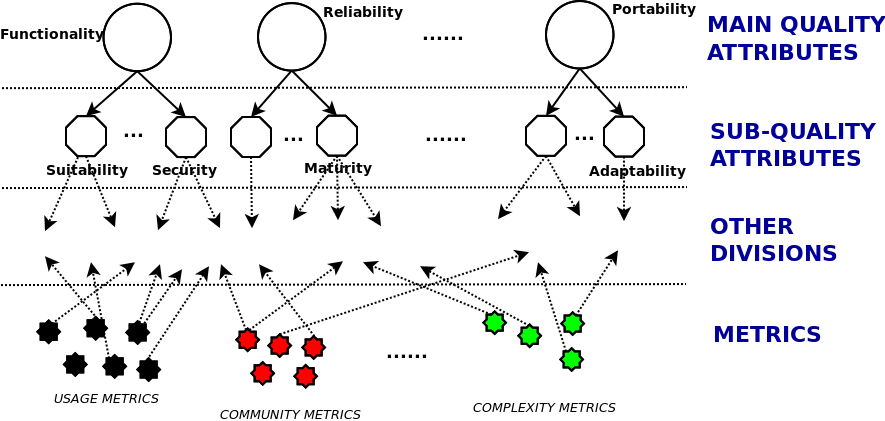
\includegraphics[scale=0.35]{figs/tree-quality-diagram.png}

\end{center}
\end{frame}


\begin{frame}
\frametitle{How to get metrics?}
\begin{center}
\begin{itemize}
 \item This is part of the automation of this quality models
 \item To be continued
\end{itemize}
\end{center}
\end{frame}


\section{Limitations}

\begin{frame}
\frametitle{Domain}
\begin{center}
\begin{itemize}
 \item Quality models are highly dependable of the domain used
 \item IDE? ERP? E-mail client?: Requirements are all different
\end{itemize}
\end{center}
\end{frame}


\begin{frame}
\frametitle{Too abstract Quality Attributes}
\begin{center}
\begin{itemize}
 \item It is not mandatory to use all of them in an evaluation of a project
 \item As we have seen, there are different points of view
 \item The ISO standard is generic enough to be partially used
 \item In fact, new attributes are added, other are modified and others are removed
\end{itemize}
\end{center}
\end{frame}


\begin{frame}
\frametitle{Objective Metrics?}
\begin{center}
\begin{itemize}
 \item Having too many metrics could derive in an unusable quality model.
 \item What about an automated quality model?
 \item Then we will face problems derived from the empirical software engineering
\end{itemize}
\end{center}
\end{frame}



\begin{frame}
\frametitle{Objective Metrics?}
\begin{center}
\begin{itemize}
 \item Are the tools we are using trustable enough?
 \item Several different data sources (tool for each one?)
 \item Different programming languages
 \item Others...
\end{itemize}
\end{center}
\end{frame}

\section{References}


\begin{frame}
\frametitle{Objective Metrics?}
\begin{center}
\begin{itemize}
\item ISO/IEC.  \textit{ISO/IEC 9126. Software engineering -- Product quality}. 2001. ISO/IEC.
\item Franch, X. and Carvallo, J. P. \textit{Using quality models in software package selection}. 2003. Software, IEEE.
\item \url{http://en.wikipedia.org/wiki/ISO/IEC_9126}
\end{itemize}
\end{center}
\end{frame}


\end{document}